Se analizará la media y el desvío estándar del potencial de membrana en reposo para dos modelos de neuronas. En el primero, las entradas se modelan como corrientes transitorias, mientras que en el segundo se modelan como cambios transitorios en la conductancia de membrana.
\section{Entradas modeladas como fuentes de corriente}
Se simula inyectar una corriente i(t) a través de un microelectrodo hacia el interior de la neurona.
El microelectrodo se puede pensar como una \textit{fuente de corriente ideal} y la membrana celular puede ser conceptualizada como si estuviera hecha por varios circuitos RC (ver figura~\ref{fig:modelo_neurona_esferica}). Como las dimensiones de la célula son muy pequeñas, el potencial en la superficie de la membrana es el mismo en todos lados. De esta manera, el comportamiento eléctrico de la célula puede ser descrito adecuadamente por un único circuito RC con una fuente de corriente (ver figura~\ref{fig:circuito_electrico_integrate_and_fire_potencial_reposo}).
\begin{figure*}[htbp!]
        \centering
        \begin{subfigure}[b]{0.45\textwidth}  
            \centering 
            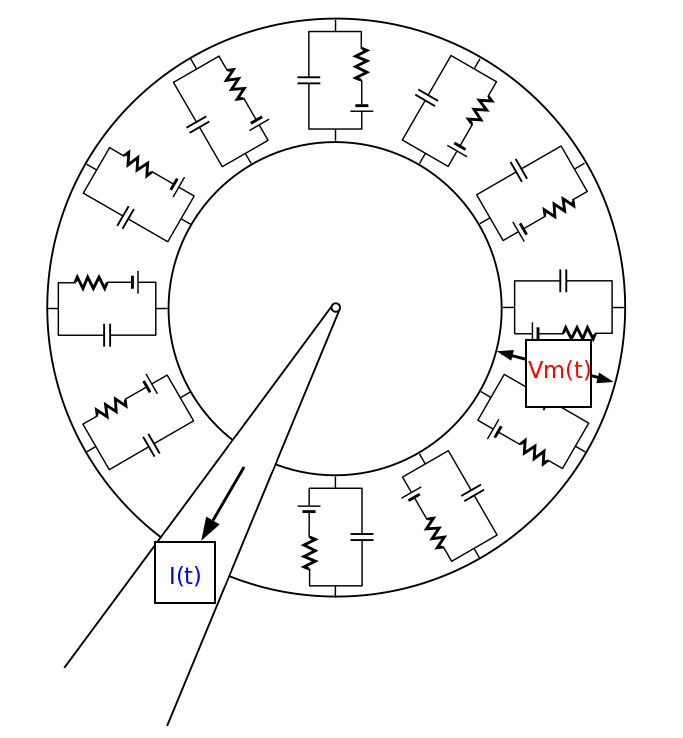
\includegraphics[width=6cm]{figures/neurona_esferica_conceptual.png}
            \caption{Modelo eléctrico de una célula esférica. Por convención, una corriente saliente es positiva, por ese motivo la flecha se dibuja así.}
            \label{fig:modelo_neurona_esferica}
        \end{subfigure}
         \hspace{0.5cm}
        \begin{subfigure}[b]{0.45\textwidth}
            \centering
            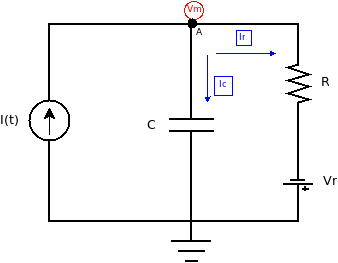
\includegraphics[width=\textwidth]{figures/integrate_fire_con_potencial_reposo.png}
            \caption{Circuito eléctrico que representa una pequeña porción de membrana. La corriente $I_r$ también es conocida como la corriente de fuga $I_l$.}
            \label{fig:circuito_electrico_integrate_and_fire_potencial_reposo}
        \end{subfigure}
        \quad
        \caption{Estructura eléctrica de una neurona}
        \label{fig:estructura_electrica_neurona}
\end{figure*}
\newpage
Siguiendo un desarrollo similar al de la sección~\ref{sec:modelo_leaky_integrate_and_fire}, pero esta vez teniendo en cuenta el potencial de reposo, la corriente que circula a través de la resistencia es:
\begin{equation}\label{eq:corriente_resistencia_fuga}
    \boxed{i_r(t)= \frac{v_m(t)-v_r}{R}}    
\end{equation}
De esta manera, se obtiene\cite{Kuhn2345}:
\begin{equation}\label{eq:ecuacion_diferncial_koch}
    \tcbhighmath[boxrule=1pt,arc=1pt,colback=blue!10!white,colframe=black]{\tau_m \dv{v_m}{t} = -\big[v_m(t) - v_r\big] + \frac{i(t)}{g_l},\ con\ v_m(0)= v_r}
\end{equation}
\begin{center}
\begin{tabular}{ r l}
\footnotesize{donde,}&\\
 \footnotesize{$v_m(t)$:}& \footnotesize{es el potencial de membrana}\\ 
 \footnotesize{i(t)}:& \footnotesize{corriente de entrada.}\\
 \footnotesize{C:}& \footnotesize{capacitancia de membrana}\\
 \footnotesize{$g_l$}:& \footnotesize{conductancia de fuga (leak)}\\
 \footnotesize{$v_r$:}& \footnotesize{potencial de reposo}
\end{tabular}
\end{center}
\subsubsection{Corriente de entrada i(t)}
La corriente i(t) es inducida por eventos sinapticos excitatorios (CEPS-Corriente excitatoria postsinaptica) e inhibitorios (CEPS - corriente inhibitoria postsinaptica) (ver sección \ref{sec:sinapsis_quimica}):
\begin{equation}
    i(t)= i_e(t) + i_i(t)=\sum_j CEPS(t-t_j) + \sum_k CIPS(t-t_k)
\end{equation}
donde, $t_j\ y\ t_k$ son los tiempos de ocurrencia de los eventos excitatorios e inhibitorios respectivamente. Se asume que estos tiempos de ocurrencia siguen una distribución Poisson:
\[t_j\sim Poi\big(\lambda_e\big) \]
\[t_k\sim Poi\big(\lambda_i\big) \]
Una CEPS y una CIPS individual se modela como funciones $\alpha$ \cite{10.5555/1137840}:
\[
    \tcbhighmath[fuzzy halo=1mm with blue!50!white,arc=2pt,
  boxrule=0pt,frame hidden]{CEPS(t)=A_e \frac{t}{\tau_e}e^{(1-t/\tau_e)}H(t)}
\]
\[
    \tcbhighmath[fuzzy halo=1mm with blue!50!white,arc=2pt,
  boxrule=0pt,frame hidden]{CIPS(t)=A_i \frac{t}{\tau_i}e^{(1-t/\tau_i)}H(t)}
\]
\begin{center}
\begin{tabular}{ r l}
 $A_e>0,\ A_i<0$:& corrientes pico\\ 
 $\tau_e,\ \tau_i$:& constantes de tiempo.
\end{tabular}
\end{center}
H(x) es la \textit{función escalón Heaviside}
\begin{equation}\label{eq:heaviside}
    H(x)= \begin{cases} 
      0 & x< 0 \\
      1 & x \geq 0 
   \end{cases}
\end{equation}
Como el sistema definido por la ecuación~\ref{eq:ecuacion_diferncial_koch} es \textit{lineal}, alcanza con conocer la respuesta de la membrana a una única corriente postsinaptica (CPS) para inferir las propiedades estadísticas causadas por múltiples CPS (bombardeo sinaptico). La respuesta a una única CPS está dada por la solución del sistema de la ecuación~\ref{eq:ecuacion_diferncial_koch} tomando i(t)=CPS(t), donde CPS(t) puede ser tanto CEPS(t) como CIPS(t).
\[
    \tcbhighmath[fuzzy halo=1mm with blue!50!white,arc=2pt,
  boxrule=0pt,frame hidden]{CPS(t)=\frac{A_s.e}{C.\tau_s}.\Bigg[\frac{-t.e^{-\frac{t}{\tau_s}}}{\frac{1}{\tau_s}-\frac{1}{\tau_m}}+\frac{e^{-\frac{t}{\tau_m}}-e^{-\frac{t}{\tau_s}}}{\big(\frac{1}{\tau_s}-\frac{1}{\tau_m}\big)^2}\Bigg].H(t)}
\]
El par $(A_s,\ \tau_s)$ puede ser tanto $(A_e,\ \tau_e)$ como $(A_i,\ \tau_i)$ \\
Como el bombardeo de potenciales de acción sigue una distribución Poisson y varias CPS se suman de manera lineal, la media $\mu(v_m)$ y la varianza $\sigma^2(v_m)$ del potencial de membrana está dado por el teorema de Campbell \cite{papoulis1991probability}:
\begin{equation}
    \tcbhighmath[boxrule=1pt,arc=1pt,colback=blue!10!white,colframe=black]{\mu(v_m)=v_r+\int CEPS(t) dt+ \lambda_i.\int CIPS(t) dt}
\end{equation}
\begin{equation}
    \tcbhighmath[boxrule=1pt,arc=1pt,colback=blue!10!white,colframe=black]{
    \sigma^2(v_m)=\lambda_e.\int CEPS^2(t) dt + \lambda_i.\int CIPS^2(t) dt
    }
\end{equation}
donde:
\[
    \tcbhighmath[fuzzy halo=1mm with blue!50!white,arc=2pt,
  boxrule=0pt,frame hidden]{\int CPS(t)dt= \frac{A_s.\tau_s.e.\tau_m}{C}}
  \]
 \[
    \tcbhighmath[fuzzy halo=1mm with blue!50!white,arc=2pt,
  boxrule=0pt,frame hidden]{\int CPS^2(t)dt= (2.\tau_m + \tau_s).\Bigg[\frac{A_s.\tau_s.e.\tau_m}{2C(\tau_m+\tau_s)}\Bigg]^2}
  \]
  